\chapter{Provably-Correct Formation Algorithm}
\label{chp:mrf2}
Follow up on the limitations of our stateless formation algorithm proposed in Chapter~\ref{chp:mrf1}, we describe a new version of a stateful formation algorithm in this Chapter.


The basic idea is to construct the desired lattice one element at a time. 
%
We simply recognize a robot's priority by identifying its ID's numerical order among the system, namely, the highest ID denotes the highest priority, the second highest ID denotes the second highest priority, and so on.
%
The robot with the highest ID acts as a ``root'' for the lattice.  
%
From there, the robot with the second highest ID moves to be a neighbor of the root robot,
assuming one of the neighbor positions defined by the lattice graph.
%
Meanwhile, other robots only move, if necessary, to maintain the connectivity
of communication graph.
%
By repeating this process, we sequentially drive one robot at a time to vacancies in the emerging formation, until all the robots are in place.
%
The primary challenges arise from the fact that each robot must execute this
strategy using only local information, and from the need to maintain
connectivity across all robots through the entire process.


The remaining sections of this chapter are organized as follows. 
%
Section~\ref{sec:vacancy} introduces the concept of vacancy used in this algorithm. 
% 
Message-passing plays an essential role for robots to interact and coordinate with each other.
%
In Section~\ref{sec:com}, we explain the communication protocols in the system.
%
That is, the procedure for each robot to generate its message periodically containing its some key global information retrieved from others' messages, such as the highest ID in the system.
%
During the algorithm execution, a spanning tree of the communication graph will be constructed by the robots for the purpose of navigation.
%
%Section~\ref{sec:sptree} describe 
Therefore, the detail of constructing a spanning tree by each robot using only local communication is also discussed in this section.
%
Furthermore, we have designed a motion strategy to ensure the connectivity of the communication graph as long as the algorithm executes in Section~\ref{sec:mov}.
%
We have proved that our algorithm guarantees the robots to form the desired pattern in finite time in Section~\ref{sec:proof}.
%
Finally, in Section~\ref{sec:exp} we evaluate our algorithm by conducting groups of simulations and comparing the results with the results using the primary approach in Chapter~\ref{chp:mrf1}.


%\clearpage
\section{Vacancy}
\label{sec:vacancy}
One side effect of the stateless formation algorithm in Chapter~\ref{chp:mrf1} is the frequent formation ``destruction'' during the algorithm executes. 
%
That is, even some robots reach positions have formed 
a lattice at time, their formation may be destroyed by other robots passing over. 


Figure~\ref{fig:destruction} shows an example, in which initially three robots $r_0, r_1, r_3$ form an authority tree, while robot $r_6$ forms another authority by itself.
%
After robots $r_0, r_1, r_3$ finish the local task assignment and reach positions, robot $r_1$ observes $r_6$.
%
Since robot $r_6$ owns the highest authority among all the robots, so these four robots reconstruct a new authority tree rooted at $r_6$. Then $r_6$ will assign tasks according to its neighbor and thus the formed lattice is destroyed.

%%%%%%%%%%%%%%%%%%%%%%%%%%%
\begin{figure}
\centering  
\begin{minipage}[b]{0.45\linewidth}
    \centering
    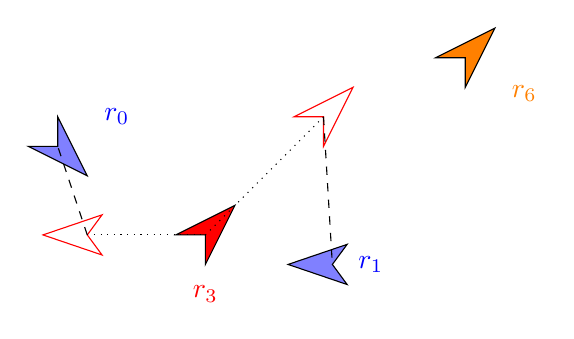
\begin{tikzpicture}[scale=1.5]
      \draw[fill=blue!50] (3,4.5) -- (2.75,5) -- (2.75,4.75) -- (2.5,4.75)   -- cycle;
      \node[color=blue] at (3.25, 5) {$r_0$};
      \draw[fill=blue!50] (5.2,3.92) -- (4.7,3.75) -- (5.2,3.58) -- (5.075,3.75)  -- cycle;
      \node[color=blue] at (5.4,3.75) {$r_1$};
      \draw[fill=red] (4,4) -- (3.75,4) -- (4.25,4.25) -- (4,3.75) -- cycle;
      \node[color=red] at (4, 3.5) {$r_3$};
      \draw[color=red] (3,4)  -- (3.125,4.17) -- (2.625,4) -- (3.125,3.83) -- cycle;
      \draw[dotted] (3,4) -- (4,4);
      \draw[color=red] (5,5) -- (4.75,5) -- (5.25,5.25) -- (5,4.75) -- cycle;
      \draw[dotted] (5,5) -- (4,4);
      \draw[dashed] (5,5) -- (5.075, 3.75);
      \draw[dashed] (3,4) -- (2.75,4.75);
      \draw[fill=orange] (6.2,5.5) -- (5.95,5.5) -- (6.45,5.75) -- (6.2,5.25)  -- cycle;
      \node[color=orange] at (6.7, 5.2) {$r_6$};
    \end{tikzpicture}
  \end{minipage}
  \begin{minipage}[b]{0.45\linewidth}
  \centering
    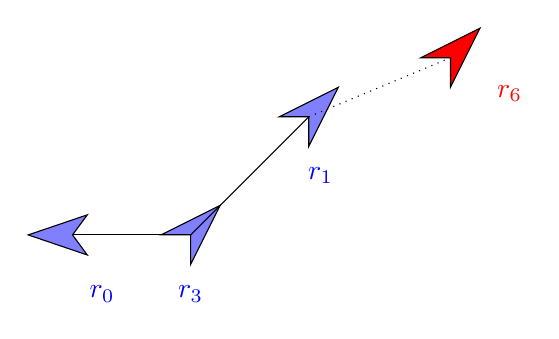
\begin{tikzpicture}[scale=1.5]
      \node[color=blue] at (3.25, 3.5) {$r_0$};
      \node[color=blue] at (5.1,4.5) {$r_1$};
      \draw[fill=blue!50] (4,4) -- (3.75,4) -- (4.25,4.25) -- (4,3.75) -- cycle;
      \node[color=blue] at (4, 3.5) {$r_3$};
      \draw[fill=blue!50] (3,4)  -- (3.125,4.17) -- (2.625,4) -- (3.125,3.83) -- cycle;
      \draw[] (3,4) -- (4,4);
      \draw[fill=blue!50] (5,5) -- (4.75,5) -- (5.25,5.25) -- (5,4.75) -- cycle;
      \draw[] (5,5) -- (4,4);
      \draw[fill=red] (6.2,5.5) -- (5.95,5.5) -- (6.45,5.75) -- (6.2,5.25)  -- cycle;
      \node[color=red] at (6.7, 5.2) {$r_6$};
      \draw[dotted] (5,5) -- (6.2,5.5);
    \end{tikzpicture}
  \end{minipage}
\caption{[left] The root robot $r_3$ assigns two positions to $r_1, r_0$, whereas robot $r_6$ is another root without any neighbor. [right] Robots $r_3, r_1, r_0$ reached assigned positions, and $r_1$ meets $r_6$ who owns the highest authority.}

\label{fig:destruction}
\end{figure}

Due to these nondeterministic destruction phenomena, it is really difficult for us to provide 
an upper bound of the algorithm execution time. 
%
In order to avoid this side effect, we want each robot to maintain a boolean state variable 
and track whether it is \textbf{stable} or \textbf{unstable}.  
%
The intuition is that stable robots remain motionless, whereas unstable robots
are either moving toward a vacancy or waiting for their turns do so.
%
Initially, each robot begins in the unstable state.
%
The unstable state changes permanently to the stable state when either the robot determines
that it has the highest ID over all robots (see Section~\ref{sec:com}), or the
robot finishes navigating to an open vacancy (see Section~\ref{sec:mov}).


The key idea of our algorithm is letting the unstable robot with the highest ID relocate itself 
to a position where it acts as a neighbor of the stable robot who owns the highest ID 
and does not yet have the maximum number of neighbors allowed by its role in the
lattice graph.

\begin{defn}
  Let $r_s$ denote a stable robot and let $u$ denote a role vertex $u$ for
  $r_s$.  For each out-edge $e_{u}^w$ of $u$ in the lattice graph, there is a
  pose $\hat{p}$ corresponding to the vertex $w$. 
  If there is no stable robot
  at $\hat{p}$, then $(\hat{p}, w)$ is a \textbf{vacancy} of $r_s$.
  (If, by chance, there is an \emph{unstable} robot at $\hat{p}$,
  we still consider $(\hat{p}, w)$ a vacancy of $r_s$.)
\end{defn}


Each stable robot periodically checks its surroundings for an open vacancy 
in terms of Algorithm~\ref{alg:vacancy}, in which the procedure of computing a vacancy for a stable robot is described. 

%%%%%%%%%%%%%%%%%%%%%%%%%%%%%%%%
\begin{algorithm}
%  \scriptsize
\SetKwInOut{Input}{input}
\SetKwInOut{Output}{output}
\Input{inMsgs, observations}
\Output{myVacancy}
   vacancies $\leftarrow \{\}$\; 
  \ForEach{outEdge of myRole}{
    pose $\leftarrow$ getPosFromTransformation(outEdge)\;
    insert Vacancy(pose, outEdge.terminal) to vacancies\;
  } 
  \ForEach{pose in vacancies}{
    \ForEach{neighborPose in observations}{
        \If{inMsgs[neighborID].stable AND neighborPose $=$ pose}{
            remove pose from vacancies\;
        }
    }
  }
  \Return vacancies.empty ? null : vacancies[0]\;
  \caption{Compute a vacancy of a stable robot}
  \label{alg:vacancy}
\end{algorithm}


Consider the lattice graph for a repeating square pattern  (Figure~\ref{fig:sq}), in Figure~\ref{fig:vacancy}, an example shows that robot $r_6$
is the stable robot with the highest ID and has three vacancies computed in terms of the
lattice graph in Figure~\ref{fig:sq}. 
%
The robot with the second highest ID $r_5$ is also stable and already a neighbor of $r_6$.
%
The unstable robot with the highest ID is robot $r_4$, which is moving toward the vacancy ahead of $r_6$.  
%
Robot $r_4$
will change its state from unstable to stable after it reaches this pose.

%%%%%%%%%%%%%%%%%%%%%%%%%%%%%%%%
\begin{figure}
  \centering
   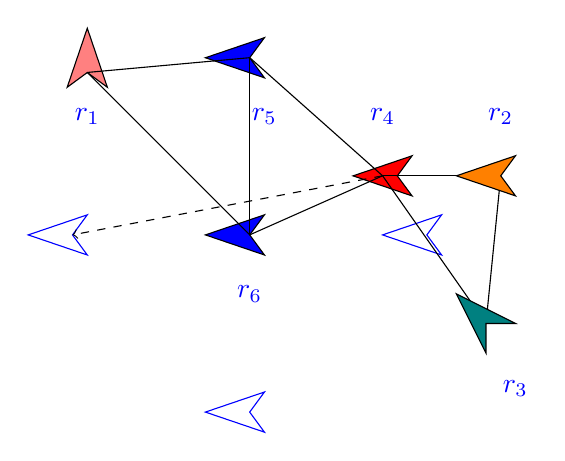
\begin{tikzpicture}[scale=1.5]
    %\useasboundingbox (1,0.5) rectangle (5.5,5);
    % center 2.875 2.75
    \coordinate (S) at (2.875, 2.75);
    \def\shifty{1}
    \def\ddy{2.5}
    \coordinate (A) at (1.5, 4.125);
    \coordinate (B) at (4,4.25-\shifty);
    \draw[fill=blue] (3,2.92) -- (2.5,2.75) -- (3,2.58) -- (2.875,2.75) -- cycle;
    \def\offset{0.5}
    \node[color=blue] at (2.875, 2.75-\offset) {$r_6$};
    % vacancies
    \def\dx{1.5}
    \def\dy{1.5}
    \draw[color=blue] (3+\dx,2.92) -- (2.5+\dx,2.75) -- (3+\dx,2.58) -- (2.875+\dx,2.75) -- cycle;
    \draw[color=blue] (3-\dx,2.92) -- (2.5-\dx,2.75) -- (3-\dx,2.58) -- (2.875-\dx,2.75) -- cycle;
    %%%%%%%
    \draw[fill=blue] (3,2.92+\dy) -- (2.5,2.75+\dy) -- (3,2.58+\dy) -- (2.875,2.75+\dy) -- cycle;
    \node[color=blue] at (3, 3.25+\offset) {$r_5$};
    %%%%%%%%
    \draw[color=blue] (3,2.92-\dy) -- (2.5,2.75-\dy) -- (3,2.58-\dy) -- (2.875,2.75-\dy) -- cycle;
    % another two robots
    \draw[fill=red!50] (1.5,4.5) -- (1.33,4) -- (1.5,4.125) -- (1.67,4) -- cycle; % center .5 4.125
    \node[color=blue] at (1.5, 3.25+\offset) {$r_1$};
    \def\shiftx{1.25}
    \draw[fill=red] (3+\shiftx,3.42) -- (2.5+\shiftx,3.25) -- (3+\shiftx,3.08) -- (2.875+\shiftx,3.25) -- cycle;          
    \node[color=blue] at (4, 4.75-\shifty) {$r_4$};
    \draw[] (S) -- (A);
    \draw[] (S) -- (B);
    \coordinate (V) at (2.875-\dx,2.75);
    \draw[dashed, ->] (B) -- (V);
    % two children of r_i
    \coordinate (C) at  (5, 3.25);
    %\draw[fill=orange] (5,3.5) -- (4.83,3) -- (5, 3.25) -- (5.17,3) -- cycle; % center .\5 3.625
    \node[color=blue] at (5, 3.75) {$r_2$};
    % center or r_c
    \def\xcc{5}
    \def\ycc{3.25}
    \def\hrlen{0.375}
    \def\ylen{0.17}
    \def\xlen{0.125}
    \coordinate (CC) at (\xcc, \ycc);
    % center of r_d
    \def\xdc{4.875}
    \def\ydc{2}
    \def\longlen{0.25}
    \coordinate (DC) at (\xdc, \ydc);
    \draw[] (B) -- (CC);
    \draw[] (B) -- (DC);
    \draw[] (CC) -- (DC);
    \coordinate (CA) at (\xcc-\hrlen, \ycc);
    \coordinate (CB) at (\xcc+\xlen, \ycc+\ylen);
    \coordinate (CD) at (\xcc+\xlen, \ycc-\ylen);
    \draw[fill=orange] (CA) -- (CB) -- (CC) -- (CD) -- cycle;
    \coordinate (D) at (5.375-\offset, 4.5-\ddy);

    \node[color=blue] at (5.125, 3.95-\ddy) {$r_3$};

  
    \coordinate (DA) at (\xdc-\longlen, \ydc+\longlen);
    \coordinate (DB) at (\xdc, \ydc-\longlen);
    \coordinate (DD) at (\xdc+\longlen, \ydc);
    \draw[fill=teal] (DA) -- (DB) -- (DC) -- (DD) -- cycle;
    
    \coordinate (R5) at (2.875, 2.75+\dy);
    \draw[] (S) -- (R5);
    \draw[] (R5) -- (A);
    \draw[] (R5) -- (B);
  \end{tikzpicture}
  \caption{Robot $r_6$ be a stable robot, it has three neighbors
    $r_1, r_5, r_4$ and three vacancies (hollow).  
    Robot $r_4$ is the relocate robot
    and its ultimate destination is the vacancy ahead of
    $r_6$. }
  
  \label{fig:vacancy}
\end{figure}
%%%%%%%%%%%%%%%%%%%%%%%%%%%%%%%%


%\clearpage
\section{Communication Procedure}
\label{sec:com}
We assume that the robots communicate by broadcasting messages to the
neighbors every $\dt$ seconds.
%
The main objective for the communication is to retrieve the principal global
information of the system and then to construct a spanning tree of the
communication graph.


The principal global information includes: 
\begin{enumerate}
\item the \textbf{highest ID} among all robots in the network;
\item the \textbf{root robot}: the stable robot who has the highest ID and at least one vacancy, it will be elected by others as the root of the spanning tree;
\item the \textbf{most important vacancy}: we order the vacancies of the root robot according to the numerical order of their corresponding vertices' IDs, then choose the first one as the most important vacancy;
%\item the highest ID among all unstable robot;
\item the \textbf{relocate robot}: the unstable robot who has the highest ID, it should relocate to the most important vacancy.
\end{enumerate}


We define a message type for robots to pass around.
%
Table~\ref{tab:msg} lists the data contained in the message for robots to acquire the principal global information. 
%
The purpose of tracing the paths from the root and the relocate robots is
to prevent the ``rumor,'' in which a robot relies upon the
information generated originally by itself.  
%
Specifically, a robot
rejects information for which its own ID appears in the
``pathFromRoot'' or ``pathFromRelocate'' lists.
%
The memory consumption for the message passing process is upper-bounded by a value linear to the number of the robots in the system. 

\begin{table}
\caption{Data included in each message.}
   \begin{tabular}{ll}
    \toprule
    \textbf{Data}  & \textbf{Description}  \\
    \midrule
    \textbf{senderID} &  ID of the robot that sent this message\\
    \midrule
    \textbf{highestID} & the highest robot ID in the system\\
    \midrule
    \textbf{rootID} &  ID of the root robot\\
    \midrule
    \textbf{relocateID} &  ID of the relocate robot\\
    \midrule
    \textbf{parentID} &  ID of the sender robot's spanning tree parent \\
    \midrule
    \textbf{vacancy} & the most important vacancy of the root robot\\
    \midrule
    \textbf{subtree} & a boolean marker showing if the sender robot is \\
        & in the subtree rooted at the relocate robot \\
    \midrule
    \textbf{stable} & a boolean label which indicates if the sender robot \\
        & is stable\\
    \midrule
    \textbf{pathFromRoot} & a list of robot IDs who are in the shortest\\
        & path to the root robot\\
    \midrule
    \textbf{pathFromRelocate} & a list of robot IDs who are in the shortest \\
        & path to the relocate robot\\
    \bottomrule
  \end{tabular}

\label{tab:msg}
\end{table}

For all the robots to reach consensus about the principal global
information, 
we set up a time parameter, called ``communication timeout'', for robots to learn about the network enough. 
%
A proper value for the communication timeout is related with the
initial distribution of the robots' poses and the shape and dimensions of the
final formation. 
%
In the worst case, the communication timeout can be bounded
above by a time linear in the number of robots.


\begin{defn}
  \label{def:timeout}
  The \textbf{communication timeout} is the number of time steps that the robot
  needs to wait before it is confident about the principal information from the
  incoming messages.
\end{defn}


Our algorithm uses the communication timeout in two related ways (Algorithm~\ref{alg:timeout}).
%
First, each robot waits until the communication timeout has passed starting from the
last change to the highest ID that the robot knew about.  
%
When this occurs,
the robot can correctly decide whether it is or is not the highest ID robot.
%
The robot that does have the highest ID can then become stable.
%
Second, the robots use the communication timeout in a similar way to identify
the unstable robot with the highest ID.  
%
This robot then becomes the relocate
robot, and begins navigating toward the most important vacancy.

\begin{algorithm}
%  \scriptsize
\SetKwInOut{Input}{input}
\SetKwInOut{Output}{output}
\Input{myPreMsg, myCurMsg, TIMEOUT}
\Output{void}
  \If{myPreMsg.highestID$\neq$ myCurMsg.highestID}{
    LAST_CHANGE_TO_HIGHEST_ID = currentTime\;
  }
  \If{myPreMsg.relocateID$\neq$ myCurMsg.relocateID}{
    LAST_CHANGE_TO_RELOCATE_ID = currentTime\;
  }
  \If{myPreMsg.rootID$\neq$ myCurMsg.rootID}{
    LAST_CHANGE_TO_ROOT_ID = currentTime\;
  }
  \If{currentTime - LAST_CHANGE_TO_HIGHEST_ID $\geq$ TIMEOUT}{
    \If{myID$=$myCurMsg.highestID}{
        I am the stable root with role 0\;
    }
  }
  \If{currentTime - LAST_CHANGE_TO_RELOCATE_ID $\geq$ TIMEOUT}{
    \If{myID$=$myCurMsg.relocateID AND I am at the vacancy pose}{
        I become stable with the role of myCurMsg.vacancy\;
    }
  }
  \caption{Update robot's knowledge with communication timeout}
  \label{alg:timeout}
\end{algorithm}

% %\clearpage
% \section{Algorithm}
% \label{sec:sptree}

During the communication process, each robot computes its message
based on the incoming messages from its neighbors. 
%
Each robot can determine the highest ID by repeatedly comparing its own ID with the highest IDs transmitted by neighbors.
%
The robots compute the highest ID unstable robot and the highest ID stable
robot with vacancy in a similar way.

Moreover, in the same communication process, the robots construct a spanning
tree of their communication graph rooted at the highest ID stable robot with
vacancy.  
%
Each robot that has at least one stable neighbor, chooses the stable neighbor that has the fewest hops from the root as its parent in this tree.
%
Each robot without stable neighbors chooses the unstable neighbor with the minimal hops to the root as its parent.  
%
A special exception, designed to reduce unnecessary movements, is that no robot chooses the relocate robot as its parent, if it has another neighbor with the same or fewer hops to the root.  
%
Ties, if any, are broken in favor of the
highest ID.  


Algorithm~\ref{alg:msg} briefly illustrates the communication process in which a robot reasons about the principle global information and its role in the spanning tree.
%
Specifically, Algorithm~\ref{alg:parent} describes the procedure for a robot to select a parent. 


Figure~\ref{fig:spanningtree} shows an example of a spanning tree of six robots.
%
Because the motion strategy uses the parent-child relationships in this
spanning tree to maintain connectivity, each robot also keeps track of whether
the relocate robot is its ancestor in the spanning tree, denoted ``subtree'' in
the message type.


\begin{algorithm}
%   % \algsetup{linenosize=\tiny}
%   \scriptsize
    \SetKwInOut{Input}{input}
    \SetKwInOut{Output}{output}
    \Input{inMsgs}
    \Output{myMsg}
    myMsg $\leftarrow$ empty message\;
    myMsg.senderID $\leftarrow$ myID\;
    myMsg.highestID $\leftarrow$ myID\;
    myMsg.stable $\leftarrow$ stable\;
    myVacancy $\leftarrow$ stable ? computeVacancy(inMsgs, observations) : null\;
    myMsg.rootID $\leftarrow$ (stable \textbf{and} myVacancy $\neq$ \textbf{null}) ? myID : INT\_MIN\;
    myMsg.relocateID $\leftarrow$ stable ? INT\_MIN : myID\;
    eligibleMsgs $\leftarrow$ \{\}\;
    vacancyFromMsgs $\leftarrow$ \textbf{null}\;
    \ForEach{msg in inMsgs}{
        myMsg.highestID $\leftarrow$ \textbf{max}(myMsg.highestID, msg.highestID)\;
        \If{\textbf{not} msg.pathFromRoot.contains(myID) \textbf{and} \textbf{not} msg.pathFromRelocate.contains(myID) }{
        insert msg into eligibleMsgs\;
        \If{msg.rootID $>$ myMsg.rootID}{
            myMsg.rootID $\leftarrow$ msg.rootID\;
            vacancyFromMsgs $\leftarrow$ msg.vacancy\;
        }
        myMsg.relocateID $\leftarrow$ \textbf{max}(myMsg.relocateID, msg.relocateID)\;
        }
    }
    minRootPath $\leftarrow$ getShortestPathFromRoot(eligibleMsgs)\;
    minRelocatePath $\leftarrow$ getShortestPathFromRelocate(eligibleMsgs)\;
    myMsg.vacancy $\leftarrow$ (myID $=$ myMsg.rootID) ? myVacancy : vacancyFromMsgs\;
    myMsg.pathFromRoot $\leftarrow$ minRootPath.append(myID)\;
    myMsg.pathFromRelocate $\leftarrow$ minRelocatePath.append(myID)\;
    \If{myID $\neq$ myMsg.rootID}{
        parentMsg $\leftarrow$ getParentMsg(eligibleMsgs, myMsg, relocateID)\;
        myMsg.parentID $\leftarrow$ parentMsg.senderID\;
        myMsg.subtree $\leftarrow$ myID $=$ myMsg.relocateID \textbf{or} parentMsg.subtree\;
    }
    \Return myMsg\;
    \caption{Compute message.}
    \label{alg:msg}
\end{algorithm}

%%%%%%%%%%%%%%%%%%%%%%%%%%%%%%%%
\begin{algorithm}
%  \scriptsize
\SetKwInOut{Input}{input}
\SetKwInOut{Output}{output}
\Input{eligibleMsgs, myMsg, relocateID}
\Output{parentMsg}
  stableMsgs $\leftarrow \{\}$\;
  myHops $\leftarrow$ myMsg.pathFromRoot.length\;
  \ForEach{msg $\mbox{in}$ eligibleMsgs}{
    \If{msg.stable}{
      insert msg to stableMsgs\;
    }
  }
  \If{!stableMsgs.empty}{
    \Return msgWithMinHops in stableMsgs\;
  }
  minHops $\leftarrow$ myHops\;
  uncleMsgs $\leftarrow \{\}$\;
  minHops $\leftarrow$ min(msg.pathFromRoot.length, minHops) \textbf{for} msg in eligibleMsgs\;
  \ForEach{msg in eligibleMsgs}{
    \If{msg.pathFromRoot.length $=$ minHops}{
        uncleMsgs $\leftarrow$ msg\;
    }
  }
  sort uncleMsgs in descending order of messages' senderIDs
  \If{myID $\neq$ relocateID AND !uncleMsgs.empty}{
    \If{uncleMsgs[0].senderID $=$ relocateID}{
        \Return uncleMsgs.size>1 ? uncleMsgs[1] : uncleMsgs[0]\;
    }
  }  
  \Return uncleMsgs.empty ? myMsg : uncleMsgs[0]\;
  \caption{Select the parent and return the parent's message.}
  \label{alg:parent}
\end{algorithm}

%%%%%%%%%%%%%%%%%%%%%%%%%%%%%%%%
\begin{figure}
   \centering
   \begin{minipage}[b]{0.45\linewidth}
  \centering
    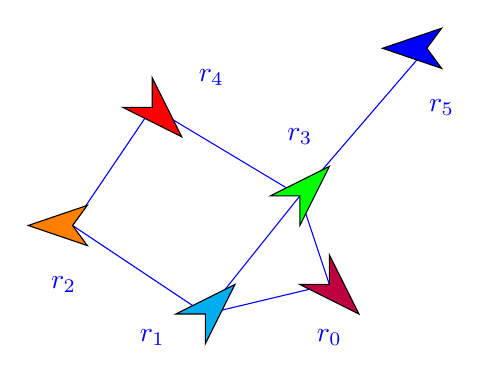
\begin{tikzpicture}[scale=1.5]
      \draw [color=blue] (4,4) -- (3.2,3); % r1--r3
      \draw [color=blue] (4,4) -- (5.075,5.25); %r3--r5
      \draw [color=blue] (4,4) -- (2.75,4.75); % r3--r4
      \draw [color=blue] (4,4) -- (4.25, 3.25); %r3--r0
      \draw [color=blue] (2.75,4.75) -- (2.075,3.75); % r4--r2
      \draw [color=blue] (3.2,3) -- (2.075,3.75); % r1--r2
      \draw [color=blue] (3.2,3) -- (4.25,3.25); %r1--r0
      \draw[fill=red] (3,4.5) -- (2.75,5) -- (2.75,4.75) -- (2.5,4.75)   -- cycle;
      \node[color=blue] at (3.25, 5) {$r_4$};
      \draw[fill=blue] (5.2,5.42) -- (4.7,5.25) -- (5.2,5.08) -- (5.075,5.25)  -- cycle;
      \node[color=blue] at (5.2,4.75) {$r_5$};
      \draw[fill=green] (4,4) -- (3.75,4) -- (4.25,4.25) -- (4,3.75) -- cycle;
      \node[color=blue] at (4, 4.5) {$r_3$};
      \draw[fill=orange] (2.2,3.92) -- (1.7,3.75) -- (2.2,3.58) -- (2.075,3.75)  -- cycle;
      \node[color=blue] at (2, 3.25) {$r_2$};
      \draw[fill=cyan] (3.2,3) -- (2.95,3) -- (3.45,3.25) -- (3.2,2.75)  -- cycle;
      \node[color=blue] at (2.75, 2.8) {$r_1$};
      \draw[fill=purple] (4.5,3) -- (4.25,3.5) -- (4.25,3.25) -- (4,3.25)   -- cycle;
      \node[color=blue] at (4.25, 2.8) {$r_0$};    
    \end{tikzpicture}
  \end{minipage}
  \begin{minipage}[b]{0.45\linewidth}
    \centering
    \begin{tikzpicture}[scale=1.5]
      \tikzstyle{every state}=[fill=purple!50, draw=none]
      \node[state, scale=0.7] (A) at (2,3) {\large{$r_5$}};
      \node[state, scale=0.7] (B) at (2,2) {\large{$r_3$}};
      \node[state, scale=0.7] (C) at (2,1) {\large{$r_1$}};
      \node[state, scale=0.7] (D) at (1,1) {\large{$r_0$}};
      \node[state, scale=0.7, fill=orange!50] (E) at (3,1) {\large{$r_4$}};
      \node[state, scale=0.6, fill=orange!50] (F) at (4,0.5) {\large{$r_2$}};
      \draw[arc] (A) to[out=-90, in=90] (B);
      \draw[arc] (B) to[out=-90, in=90] (C);
      \draw[arc] (B) to[out=-135, in=45] (D);
      \draw[arc] (B) to[out=-45, in=135] (E);
      \draw[arc] (E) to[out=-25, in=150] (F);
    \end{tikzpicture}
  \end{minipage}
\caption{[left] Communication graph of six robots. [right] Assume
  $r_5$ has the highest stable ID and a vacancy. A spanning tree
  corresponding to the left communication graph is built, in which the
  root is $r_5$. Let $r_4$ be the relocate robot, it then is the root
  of the moving subtree, in which $r_2$ is its descendant.}

   \label{fig:spanningtree}
\end{figure}
%%%%%%%%%%%%%%%%%%%%%%%%%%%%%%%

%\clearpage
\section{Movement Strategy}
\label{sec:mov}

Similar to the previous method in Chapter~\ref{chp:mrf1}, we use the bounded movement idea from Lemma~\ref{lem:boundedrange} to maintain
the connection between two robots if there exists a parent-child relationship
between them in the tree structure.  
%
The intuition is, only the relocate robot and its descendants (if any) move, while ensuring no one falls disconnected with others in the system.
%
A key difference from the prior algorithm is an inversion of responsibility:
rather than tasking each robot in this subtree to remain within range of its
parent, we instead require each parent to obey a ``No Child Left Behind
(NCLB)'' policy, which allows only movements that are guaranteed to stay within
bounded range of each of its children.
%
In turn, each child moves close enough to its parent to enable the parent to
make progress in spite of the NCLB constraint.
%
Specifically, each moving robot computes in the intersection of of the bounded
ranges of its children.  
%
This intersection region forms a ``safe region'' such
that if the robot stays with its safe region, it can guarantee to remain within
range of all of its children in the next time step.  
%
A robot that stays within
its safe region is said to obey NCLB.


Recall the scenario in Figure~\ref{fig:vacancy}, robot $r_4$ is moving towards to the vacancy ahead of robot $r_6$. 
%
With the NCLB policy, robot $r_4$ computes an intermediate goal $g_4$ within the safe region of $r_2, r_3$ (shaded region), since it is an ascendant of the two robots, as shown in Figure~\ref{fig:nclb}.

The movement strategy is divided into three cases.
\begin{enumerate}
  \item If a robot is stable, or it is not in the moving subtree, then it does
  not move.

  \item If a robot is the relocate robot, it moves
  toward its parent, unless its parent is the root, in which case it moves
  toward the vacancy, without violating NCLB.
  % 
  Figure~\ref{fig:nclb} shows a scenario in which a relocate robot
  computes an intermediate goal according to the bounded ranges of its
  children.

  \item For other robots in the moving subtree, we set a ``safe distance'',
  denoted $d_s \in (0, \range-v\dt)$.  If the robot is within distance $d_s$ of
  its parent, it does not move.  Otherwise, moves it directly toward its parent
  while staying within its NCLB safe region.
  %
\end{enumerate}

A special case occurs if the safe region for any robot is empty.
%
In that case, the robot does not move.  
%
We can still guarantee connectivity in this case
because the children (which must exist to get an empty safe region) will only
move toward the robot.  
%
Movements that decrease the distance between robots
cannot break their connectivity.  
%
If \hbox{$d_s < \range - v\dt$}, then the safe
region will eventually be non-empty (Figure~\ref{fig:safedist2}).

Figure~\ref{fig:safedist} gives another example of the NCLB movement strategy,
in which the relocate robot $r_4$ first waits for its child $r_2$ to come closer, then
computes its intermediate goal $g_4$ in the bounded range $B_2$ of its children.


In this way, the relocate robot navigates to the vacancy by tracing its path to the root.  
%
It then changes its
state from unstable to stable, triggering the communication process to identify
the next relocate robot and the next vacancy.  
%
After each robot has moved to a
vacancy, the formation is complete, and the algorithm terminates upon
discovering that no unstable robots remain.

%%%%%%%%%%%%%%%%%%%%%%%%%%%%%%%%
\begin{figure}
\centering
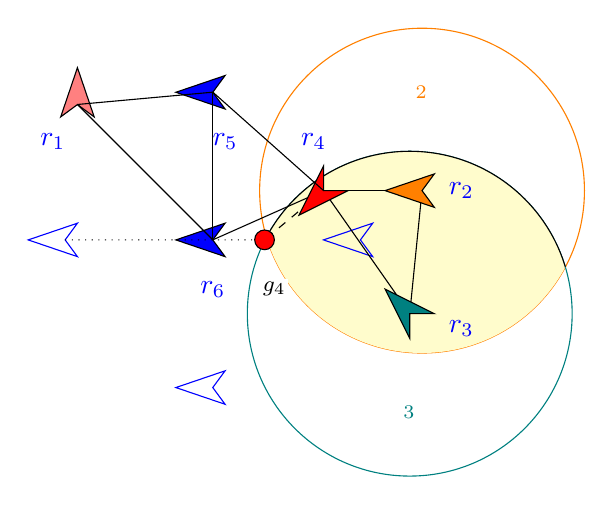
\begin{tikzpicture}[scale=1.25]
    \tikzstyle{ann} = [fill=white, font=\footnotesize,inner sep=1pt]   
    %\useasboundingbox (1,0.5) rectangle (5.5,5);
    % center 2.875 2.75
    \def\xs{2.875}
    \def\ys{2.75}
    \coordinate (S) at (\xs, \ys);
    \def\shiftx{1.25}               
    \def\shifty{1}
    \def\ddy{2.5}
    \def\offset{0.5}
    \def\movedist{1.65}
    \coordinate (A) at (1.5, 4.125);
    \coordinate (B) at (4,4.25-\shifty); % r_i
    \def\xrc{5}
    \def\yrc{3.25}
    \coordinate (C) at (\xrc, \yrc);
    \def\xrd{4.875}
    \def\yrd{2}
    \coordinate (D) at (\xrd, \yrd);
     % ranges of r_c and r_d
    \def\childcircleD{(D) circle (\movedist)}
    \def\childcircleC{(C) circle (\movedist)}
    \draw[orange] \childcircleC;
    \draw[teal] \childcircleD;
    % intersection region of children's ranges
    \begin{scope}
      \clip \childcircleC;
      \filldraw[fill=yellow!20] \childcircleD;
    \end{scope}
    
    \draw[fill=blue] (3,2.92) -- (2.5,2.75) -- (3,2.58) -- (2.875,2.75) -- cycle;
    \node[color=blue] at (2.875, 2.75-\offset) {$r_6$};
    \draw[fill=red!50] (1.5,4.5) -- (1.33,4) -- (1.5,4.125) -- (1.67,4) -- cycle; % center .5 4.125
    % vacancies
    \def\dx{1.5}
    \def\dy{1.5}
    \draw[color=blue] (3+\dx,2.92) -- (2.5+\dx,2.75) -- (3+\dx,2.58) -- (2.875+\dx,2.75) -- cycle;
    \draw[color=blue] (3-\dx,2.92) -- (2.5-\dx,2.75) -- (3-\dx,2.58) -- (2.875-\dx,2.75) -- cycle;
   % \draw[color=blue] (3,2.92+\dy) -- (2.5,2.75+\dy) -- (3,2.58+\dy) -- (2.875,2.75+\dy) -- cycle;
    %%%%%%%
    \draw[fill=blue] (3,2.92+\dy) -- (2.5,2.75+\dy) -- (3,2.58+\dy) -- (2.875,2.75+\dy) -- cycle;
    \node[color=blue] at (3, 3.25+\offset) {$r_5$};
    %%%%%%%%
    \draw[color=blue] (3,2.92-\dy) -- (2.5,2.75-\dy) -- (3,2.58-\dy) -- (2.875,2.75-\dy) -- cycle;
   
    \node[color=blue] at (1.25, 3.25+\offset) {$r_1$};
    %%%%%%%%%%%%%%%% triangle facing -135 degree
    \def\xc{4}
    \def\yc{3.25}
    \coordinate (TC) at (\xc, \yc);
    \def\longlen{0.25}
    \coordinate (TA) at (\xc-\longlen, \yc-\longlen);
    \coordinate (TB) at (\xc, \yc+\longlen);
    \coordinate (TD) at (\xc+\longlen, \yc);
 
    %%%%%%%%%%%%%%%%%%%%%%%%%%%%%%%%%%%%%%%%%%%%%
    \node[color=blue] at (3.9, 4.75-\shifty) {$r_4$};
    \draw[] (S) -- (A);
    \draw[] (S) -- (B);
  
    \node[color=blue] at (5.4, 3.25) {$r_2$};
    \draw[] (B) -- (C);
   
    \node[color=blue] at (5.4, 4.35-\ddy) {$r_3$};
    \draw[] (B) -- (D);
    \draw[] (C) -- (D);
    \coordinate (G) at (1.9+\dx,2.75);
    \draw[dotted] (2.875-\dx,2.75) -- (G);
    \draw[dashed] (B) -- (G);
    \def\goalcircleG{(G) circle (0.1)}
    \draw[fill=red] \goalcircleG;
    \node[ann] at (3.5,2.25) {$g_4$};
    % three robots
    \draw[fill=red] (TA) -- (TB) -- (TC) -- (TD) -- cycle;
    % draw r_c
    \def\xcc{5}
    \def\ycc{3.25}
    \def\hrlen{0.375}
    \def\ylen{0.17}
    \def\xlen{0.125}
    \coordinate (CC) at (\xcc, \ycc);
    \coordinate (CA) at (\xcc-\hrlen, \ycc);
    \coordinate (CB) at (\xcc+\xlen, \ycc+\ylen);
    \coordinate (CD) at (\xcc+\xlen, \ycc-\ylen);
    \draw[fill=orange] (CA) -- (CB) -- (CC) -- (CD) -- cycle;
    %\def\parentCircle {(S) circle (\movedist)}
    %\draw[color=blue] \parentCircle;
    % draw r_d  heading 135 degrees
    \def\xdc{4.875}
    \def\ydc{2}
    \coordinate (DC) at (\xdc, \ydc);
    \coordinate (DA) at (\xdc-\longlen, \ydc+\longlen);
    \coordinate (DB) at (\xdc, \ydc-\longlen);
    \coordinate (DD) at (\xdc+\longlen, \ydc);
    \draw[fill=teal] (DA) -- (DB) -- (DC) -- (DD) -- cycle;
    %%%%%%%%%%%%%% add texts of bounded ranges
    %\node[color=blue] at (\xs-0.75, \ys-\shifty) {$\B_s$};
    \node[color=orange] at (\xrc, \yrc+\shifty) {$\B_2$};    
    \node[color=teal] at (\xrd, \yrd-\shifty) {$\B_3$};
    
    \coordinate (R5) at (2.875, 2.75+\dy);
    \draw[] (S) -- (R5);
    \draw[] (R5) -- (A);
    \draw[] (R5) -- (B);
  \end{tikzpicture}
  \caption{The relocate robot $r_4$ has two descendants $r_2,
    r_3$ in the moving subtree. Two circles denote the bounded
    ranges of $r_2, r_3$, $r_4$ finds an intermediate goal (red dot)
    $g_4\in\left(\B_3 \cap \B_3\right)$.}
\label{fig:nclb}
\end{figure}
%%%%%%%%%%%%%%%%%%%%%%%%%%%%%%%%
\begin{figure}
\centering
\begin{minipage}{0.9\linewidth}
  \centering
  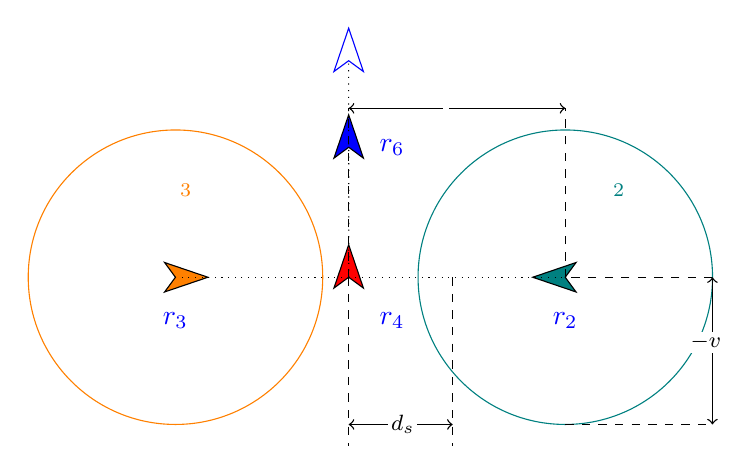
\begin{tikzpicture}[scale=1.1]
    \tikzstyle{ann} = [fill=white,font=\footnotesize,inner sep=1pt]
    % \useasboundingbox (1,0.5) rectangle (5.5,5);
    % center 2.875 2.75
    \coordinate (S) at (2.875, 2.75);
    \def\offset{0.5}
    \draw[fill=orange] (2.75,2.92) -- (3.25,2.75) -- (2.75,2.58) -- (2.875,2.75) -- cycle;
    \node[color=blue] at (2.875, 2.75-\offset) {$r_3$};
    \node[color=orange] at (3,3.75) {$\B_3$}; 
    % vacancy
    \def\dx{1.5}
    \def\ddx{2}
    \def\dddx{4.5}
    \coordinate (I) at (2.875+\ddx,2.75);
    \coordinate (C) at (2.875+\dddx,2.75);
    % \draw[color=blue] (3-\dx,2.92) -- (2.5-\dx,2.75) -- (3-\dx,2.58) -- (2.875-\dx,2.75) -- cycle;
    %\draw[fill=red] (3+\ddx,2.92) -- (2.5+\ddx,2.75) -- (3+\ddx,2.58) -- (2.875+\ddx,2.75) -- cycle;
    \draw[fill=red] (4.875, 3.125) -- (4.705,2.625) -- (4.875, 2.75) -- (5.045,2.625) -- cycle; 
    \node[color=blue] at (4.875+\offset, 2.75-\offset) {$r_4$};
    \draw[fill=teal] (3+\dddx,2.92) -- (2.5+\dddx,2.75) -- (3+\dddx,2.58) -- (2.875+\dddx,2.75) -- cycle;
    \node[color=blue] at (7.375, 2.75-\offset) {$r_2$};
    \draw[dotted] (I) -- (S);
    \draw[dotted] (I) -- (C);

    \def\rd{4}
    \coordinate (R3) at (4.875, 4.25);
    %\draw[fill=orange] (1.5,4.5) -- (1.33,4) -- (1.5,4.125) -- (1.67,4) -- cycle; % center .5 4.125
    \draw[fill=blue] (4.875, 0.625+\rd) -- (4.705,0.125+\rd) -- (R3) -- (5.045,0.125+\rd) -- cycle; 
    \node[color=blue] at (4.875+\offset, 4.25) {$r_6$};
    
    \draw[color=blue] (4.875, 5.625) -- (4.705,5.125) -- (4.875,5.25) -- (5.045,5.125) -- cycle; 
    \draw[dotted] (I) -- (4.875,5.25);

    \def\safedist{1.2}
    \def\circleSafeI {(I) circle (\safedist)}
    %\draw[color=red] \circleSafeI;
    \def\movedist{1.7}
    \def\circleMoveC {(C) circle (\movedist)}
    \def\circleMoveS {(S) circle (\movedist)}
    \draw[color=teal] \circleMoveC;
    \draw[color=orange] \circleMoveS;
    % radius of circleMoveC
    \draw[dashed,line width=.5pt] (7.375, 2.75-\movedist) -- (7.375+\movedist,2.75-\movedist);
    \draw[dashed,line width=.5pt] (7.375+\movedist, 2.75) -- (7.375, 2.75);
    \draw[arrows=<->,line width=.5pt] (7.375+\movedist,2.75-\movedist) -- (7.375+\movedist,2.75);
    \node[ann] at (9,2) {$\range-v\dt$};
    \coordinate (Cu) at (7.375, 3+\movedist);
    \coordinate (Iu) at (4.875, 3+\movedist);
    \draw[dashed, line width=.5pt] (C) -- (Cu);
    \draw[dashed, line width=.5pt] (I) -- (Iu);
    \draw[arrows=<->, line width=.5pt] (Cu) -- (Iu);
    \node[ann] at (6, 3+\movedist) {$\range$};
    \coordinate (Id) at (4.875, 2.5-\movedist);
    \coordinate (M) at (4.875+\safedist, 2.75);
    \coordinate (Md) at (4.875+\safedist, 2.5-\movedist);
    \draw[dashed, line width=.5pt] (I) -- (Id);
    \draw[dashed, line width=.5pt] (M) -- (Md);
    \coordinate (Id2) at (4.875, 2.75-\movedist);
    \coordinate (Md2) at (4.875+\safedist, 2.75-\movedist);
    \draw[arrows=<->, line width=.5pt] (Id2) -- (Md2);
    \node[ann] at (5.5, 2.75-\movedist) {$d_s$};
    %%%%
    % \def\parentCircle {(S) circle (\movedist)}
    % \draw[color=blue] \parentCircle;
    % \node[color=blue] at (3,3.75) {$\B_s$};
    \node[color=teal] at (8,3.75) {$\B_2$}; 
        %%%%           
    %% \coordinate (X) at (3.5-\dx, 2.75);
    %% \coordinate (Xd) at (3.5-\dx,2.75-\movedist);
    %% \draw[arrows=<->, line width=.5pt] (X) -- (Xd);
    %% \node[ann] at (1.75,2) {$\range-v\dt$};
    %% \coordinate (Sd) at (2.875, 2.75-\movedist);
    %% \draw[dashed,line width=.5pt] (Xd) -- (Sd);
    %% \draw[dashed,line width=.5pt] (S) -- (X);
  \end{tikzpicture}
\end{minipage}
\begin{minipage}{0.9\linewidth}
  \centering
   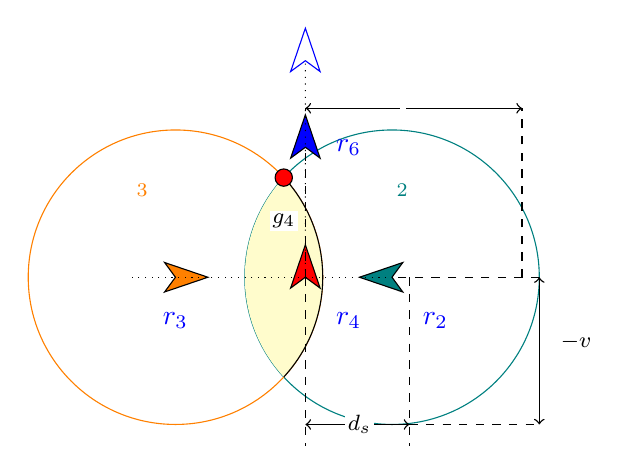
\begin{tikzpicture}[scale=1.1]
    \tikzstyle{ann} = [fill=white,font=\footnotesize,inner sep=1pt]
    % \useasboundingbox (1,0.5) rectangle (5.5,5);
    % center 2.875 2.75
    \coordinate (S) at (2.875, 2.75);
    \def\offset{0.5}
    \draw[fill=orange] (2.75+\offset,2.92) -- (3.25+\offset,2.75) -- (2.75+\offset,2.58) -- (2.875+\offset,2.75) -- cycle;
    \node[color=blue] at (2.875+\offset, 2.75-\offset) {$r_3$};
    \node[color=orange] at (3,3.75) {$\B_3$}; 
    \coordinate (D) at (2.875+\offset, 2.75);
    
    % vacancy
    \def\dx{1.5}
    \def\ddx{2}
    \def\dddx{3}
    \coordinate (I) at (2.875+\ddx,2.75);  %4.375, 2.75
    \coordinate (C) at (2.875+\dddx,2.75); %5.875, 2.75
    \def\safedist{1.2}
    \def\circleSafeI {(I) circle (\safedist)}
    %\draw[color=red] \circleSafeI;
    \def\movedist{1.7}
    \def\circleMoveC {(C) circle (\movedist)}
    \draw[color=teal] \circleMoveC;
    \def\circleMoveD {(D) circle (\movedist)}
    \draw[color=orange] \circleMoveD;
    \begin{scope}
      \clip \circleMoveC;
      \filldraw[fill=yellow!20] \circleMoveD;
    \end{scope}
    %\draw[color=blue] (3-\dx,2.92) -- (2.5-\dx,2.75) -- (3-\dx,2.58) -- (2.875-\dx,2.75) -- cycle;
    %\draw[fill=red] (3+\ddx,2.92) -- (2.5+\ddx,2.75) -- (3+\ddx,2.58) -- (2.875+\ddx,2.75) -- cycle;
    \draw[fill=red] (4.875, 3.125) -- (4.705,2.625) -- (4.875, 2.75) -- (5.045,2.625) -- cycle; 
    \node[color=blue] at (4.875+\offset, 2.75-\offset) {$r_4$};
    \draw[fill=teal] (3+\dddx,2.92) -- (2.5+\dddx,2.75) -- (3+\dddx,2.58) -- (2.875+\dddx,2.75) -- cycle;
    \node[color=blue] at (5.875+\offset, 2.75-\offset) {$r_2$};
    \draw[dotted] (I) -- (S);
    \draw[dotted] (I) -- (C);

    %%%%%%%%%%%%%%%%
    \coordinate (Cu) at (7.375, 3+\movedist);
    \coordinate (Iu) at (4.875, 3+\movedist);
    \coordinate (Co) at (7.375, 2.75);
    \draw[dashed, line width=.5pt] (Co) -- (Cu);
    \draw[dashed, line width=.5pt] (I) -- (Iu);
    \draw[arrows=<->, line width=.5pt] (Cu) -- (Iu);
    \node[ann] at (6, 3+\movedist) {$\range$};
    \coordinate (Id) at (4.875, 2.5-\movedist);
    \coordinate (M) at (4.875+\safedist, 2.75);
    \coordinate (Md) at (4.875+\safedist, 2.5-\movedist);
    \draw[dashed, line width=.5pt] (I) -- (Id);
    \draw[dashed, line width=.5pt] (M) -- (Md);
    \coordinate (Id2) at (4.875, 2.75-\movedist);
    \coordinate (Md2) at (4.875+\safedist, 2.75-\movedist);
    \draw[arrows=<->, line width=.5pt] (Id2) -- (Md2);
    \node[ann] at (5.5, 2.75-\movedist) {$d_s$};
    %%%%%%%%%%%%%%%%%
    \coordinate (N) at (5.875+\movedist, 2.75);
    \coordinate (Nd) at (5.875+\movedist, 2.75-\movedist);
    \draw[dashed,line width=.5pt] (N) -- (C);
    \draw[dashed,line width=.5pt] (Md2) -- (Nd);
    % radius of circleMoveC
    \draw[arrows=<->,line width=.5pt] (N) -- (Nd);
    \node[ann] at (8,2) {$\range-v\dt$};
    %%%% G.x = c.x - \movedist
    \coordinate (G) at (4.625, 3.9);
    \draw[fill=red] (G) circle (0.1);
    \node[ann] at (4.625, 3.9-\offset) {$g_4$};
    %%%%
    % \def\parentCircle {(S) circle (\movedist)}
    % \draw[color=blue] \parentCircle;
    %%%%
    %\node[color=blue] at (3,3.75) {$\B_s$};
    \node[color=teal] at (6,3.75) {$\B_2$}; 
    %% \coordinate (X) at (3.5-\dx, 2.75);
    %% \coordinate (Xd) at (3.5-\dx,2.75-\movedist);
    %% \draw[arrows=<->, line width=.5pt] (X) -- (Xd);
    %% \node[ann] at (1.75,2) {$\range-v\dt$};
    %% \coordinate (Sd) at (2.875, 2.75-\movedist);
    %% \draw[dashed,line width=.5pt] (Xd) -- (Sd);
    %% \draw[dashed,line width=.5pt] (S) -- (X);
    \def\rd{4}
    \coordinate (R3) at (4.875, 4.25);
    %\draw[fill=orange] (1.5,4.5) -- (1.33,4) -- (1.5,4.125) -- (1.67,4) -- cycle; % center .5 4.125
    \draw[fill=blue] (4.875, 0.625+\rd) -- (4.705,0.125+\rd) -- (R3) -- (5.045,0.125+\rd) -- cycle; 
    \node[color=blue] at (4.875+\offset, 4.25) {$r_6$};
    
    \draw[color=blue] (4.875, 5.625) -- (4.705,5.125) -- (4.875,5.25) -- (5.045,5.125) -- cycle; 
    \draw[dotted] (I) -- (4.875,5.25);
    
    \end{tikzpicture}
\end{minipage}
   \caption{(top) The relocate robot $r_4$ intends to move to the
   vacancy (hollow arrow) of the root robot $r_6$. Robots $r_2, r_3$ are 
   children of $r_4$. Since $\B_2\cap\B_2=\emptyset$, $r_4$
   waits for $r_2, r_3$ to move close to it. (bottom) When
   the safe region for $r_4$ becomes non-empty, the relocate robot $r_4$
   finds the closest point $g_4 \in \B_2\cap\B_3$ (red dot)
   to the vacancy as an intermediate goal.}
\label{fig:safedist2}
\end{figure}
%%%%%%%%%%%%%%%%%%%%%%%%%%%%%%%%
\begin{figure}
\centering
\begin{minipage}{0.9\linewidth}
  \centering
  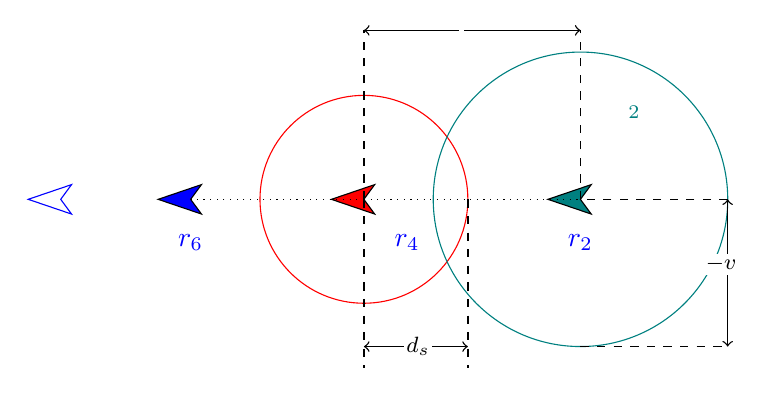
\begin{tikzpicture}[scale=1.1]
    \tikzstyle{ann} = [fill=white,font=\footnotesize,inner sep=1pt]
    % \useasboundingbox (1,0.5) rectangle (5.5,5);
    % center 2.875 2.75
    \coordinate (S) at (2.875, 2.75);
    \def\offset{0.5}
    \draw[fill=blue] (3,2.92) -- (2.5,2.75) -- (3,2.58) -- (2.875,2.75) -- cycle;
    \node[color=blue] at (2.875, 2.75-\offset) {$r_6$};
    % vacancy
    \def\dx{1.5}
    \def\ddx{2}
    \def\dddx{4.5}
    \coordinate (I) at (2.875+\ddx,2.75);
    \coordinate (C) at (2.875+\dddx,2.75);
    \draw[color=blue] (3-\dx,2.92) -- (2.5-\dx,2.75) -- (3-\dx,2.58) -- (2.875-\dx,2.75) -- cycle;
    \draw[fill=red] (3+\ddx,2.92) -- (2.5+\ddx,2.75) -- (3+\ddx,2.58) -- (2.875+\ddx,2.75) -- cycle;
    \node[color=blue] at (4.875+\offset, 2.75-\offset) {$r_4$};
    \draw[fill=teal] (3+\dddx,2.92) -- (2.5+\dddx,2.75) -- (3+\dddx,2.58) -- (2.875+\dddx,2.75) -- cycle;
    \node[color=blue] at (7.375, 2.75-\offset) {$r_2$};
    \draw[dotted] (I) -- (S);
    \draw[dotted] (I) -- (C);

    \def\safedist{1.2}
    \def\circleSafeI {(I) circle (\safedist)}
    \draw[color=red] \circleSafeI;
    \def\movedist{1.7}
    \def\circleMoveC {(C) circle (\movedist)}
    \draw[color=teal] \circleMoveC;
    % radius of circleMoveC
    \draw[dashed,line width=.5pt] (7.375, 2.75-\movedist) -- (7.375+\movedist,2.75-\movedist);
    \draw[dashed,line width=.5pt] (7.375+\movedist, 2.75) -- (7.375, 2.75);
    \draw[arrows=<->,line width=.5pt] (7.375+\movedist,2.75-\movedist) -- (7.375+\movedist,2.75);
    \node[ann] at (9,2) {$\range-v\dt$};
    \coordinate (Cu) at (7.375, 3+\movedist);
    \coordinate (Iu) at (4.875, 3+\movedist);
    \draw[dashed, line width=.5pt] (C) -- (Cu);
    \draw[dashed, line width=.5pt] (I) -- (Iu);
    \draw[arrows=<->, line width=.5pt] (Cu) -- (Iu);
    \node[ann] at (6, 3+\movedist) {$\range$};
    \coordinate (Id) at (4.875, 2.5-\movedist);
    \coordinate (M) at (4.875+\safedist, 2.75);
    \coordinate (Md) at (4.875+\safedist, 2.5-\movedist);
    \draw[dashed, line width=.5pt] (I) -- (Id);
    \draw[dashed, line width=.5pt] (M) -- (Md);
    \coordinate (Id2) at (4.875, 2.75-\movedist);
    \coordinate (Md2) at (4.875+\safedist, 2.75-\movedist);
    \draw[arrows=<->, line width=.5pt] (Id2) -- (Md2);
    \node[ann] at (5.5, 2.75-\movedist) {$d_s$};
    %%%%
    % \def\parentCircle {(S) circle (\movedist)}
    % \draw[color=blue] \parentCircle;
    % \node[color=blue] at (3,3.75) {$\B_s$};
    \node[color=teal] at (8,3.75) {$\B_2$}; 
        %%%%           
    %% \coordinate (X) at (3.5-\dx, 2.75);
    %% \coordinate (Xd) at (3.5-\dx,2.75-\movedist);
    %% \draw[arrows=<->, line width=.5pt] (X) -- (Xd);
    %% \node[ann] at (1.75,2) {$\range-v\dt$};
    %% \coordinate (Sd) at (2.875, 2.75-\movedist);
    %% \draw[dashed,line width=.5pt] (Xd) -- (Sd);
    %% \draw[dashed,line width=.5pt] (S) -- (X);
  \end{tikzpicture}
\end{minipage}
\begin{minipage}{0.9\linewidth}
  \centering
   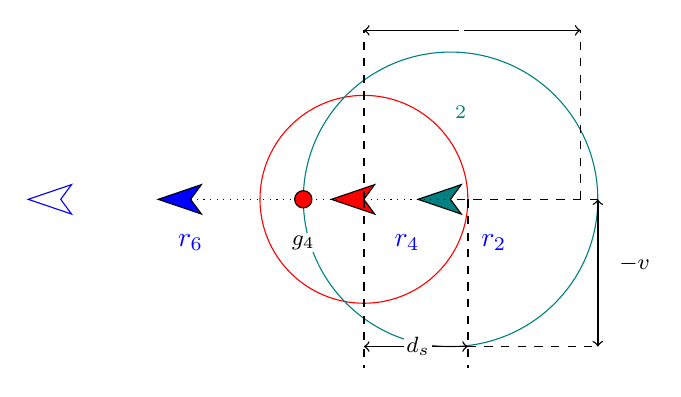
\begin{tikzpicture}[scale=1.1]
    \tikzstyle{ann} = [fill=white,font=\footnotesize,inner sep=1pt]
    % \useasboundingbox (1,0.5) rectangle (5.5,5);
    % center 2.875 2.75
    \coordinate (S) at (2.875, 2.75);
    \def\offset{0.5}
    \draw[fill=blue] (3,2.92) -- (2.5,2.75) -- (3,2.58) -- (2.875,2.75) -- cycle;
    \node[color=blue] at (2.875, 2.75-\offset) {$r_6$};
    % vacancy
    \def\dx{1.5}
    \def\ddx{2}
    \def\dddx{3}
    \coordinate (I) at (2.875+\ddx,2.75);  %4.375, 2.75
    \coordinate (C) at (2.875+\dddx,2.75); %5.875, 2.75
    \draw[color=blue] (3-\dx,2.92) -- (2.5-\dx,2.75) -- (3-\dx,2.58) -- (2.875-\dx,2.75) -- cycle;
    \draw[fill=red] (3+\ddx,2.92) -- (2.5+\ddx,2.75) -- (3+\ddx,2.58) -- (2.875+\ddx,2.75) -- cycle;
    \node[color=blue] at (4.875+\offset, 2.75-\offset) {$r_4$};
    \draw[fill=teal] (3+\dddx,2.92) -- (2.5+\dddx,2.75) -- (3+\dddx,2.58) -- (2.875+\dddx,2.75) -- cycle;
    \node[color=blue] at (5.875+\offset, 2.75-\offset) {$r_2$};
    \draw[dotted] (I) -- (S);
    \draw[dotted] (I) -- (C);

    \def\safedist{1.2}
    \def\circleSafeI {(I) circle (\safedist)}
    \draw[color=red] \circleSafeI;
    \def\movedist{1.7}
    \def\circleMoveC {(C) circle (\movedist)}
    \draw[color=teal] \circleMoveC;
    %%%%%%%%%%%%%%%%
    \coordinate (Cu) at (7.375, 3+\movedist);
    \coordinate (Iu) at (4.875, 3+\movedist);
    \coordinate (Co) at (7.375, 2.75);
    \draw[dashed, line width=.5pt] (Co) -- (Cu);
    \draw[dashed, line width=.5pt] (I) -- (Iu);
    \draw[arrows=<->, line width=.5pt] (Cu) -- (Iu);
    \node[ann] at (6, 3+\movedist) {$\range$};
    \coordinate (Id) at (4.875, 2.5-\movedist);
    \coordinate (M) at (4.875+\safedist, 2.75);
    \coordinate (Md) at (4.875+\safedist, 2.5-\movedist);
    \draw[dashed, line width=.5pt] (I) -- (Id);
    \draw[dashed, line width=.5pt] (M) -- (Md);
    \coordinate (Id2) at (4.875, 2.75-\movedist);
    \coordinate (Md2) at (4.875+\safedist, 2.75-\movedist);
    \draw[arrows=<->, line width=.5pt] (Id2) -- (Md2);
    \node[ann] at (5.5, 2.75-\movedist) {$d_s$};
    %%%%%%%%%%%%%%%%%
    \coordinate (N) at (5.875+\movedist, 2.75);
    \coordinate (Nd) at (5.875+\movedist, 2.75-\movedist);
    \draw[dashed,line width=.5pt] (N) -- (C);
    \draw[dashed,line width=.5pt] (Md2) -- (Nd);
    % radius of circleMoveC
    \draw[arrows=<->,line width=.5pt] (N) -- (Nd);
    \node[ann] at (8,2) {$\range-v\dt$};
    %%%% G.x = c.x - \movedist
    \coordinate (G) at (5.875-\movedist, 2.75);
    \draw[fill=red] (G) circle (0.1);
    \node[ann] at (5.875-\movedist, 2.75-\offset) {$g_4$};
    %%%%
    % \def\parentCircle {(S) circle (\movedist)}
    % \draw[color=blue] \parentCircle;
    %%%%
    %\node[color=blue] at (3,3.75) {$\B_s$};
    \node[color=teal] at (6,3.75) {$\B_2$}; 
    %% \coordinate (X) at (3.5-\dx, 2.75);
    %% \coordinate (Xd) at (3.5-\dx,2.75-\movedist);
    %% \draw[arrows=<->, line width=.5pt] (X) -- (Xd);
    %% \node[ann] at (1.75,2) {$\range-v\dt$};
    %% \coordinate (Sd) at (2.875, 2.75-\movedist);
    %% \draw[dashed,line width=.5pt] (Xd) -- (Sd);
    %% \draw[dashed,line width=.5pt] (S) -- (X);
    \end{tikzpicture}
\end{minipage}
   \caption{(top) The relocate robot $r_4$ intends to move to the
   vacancy (hollow arrow) of the root robot $r_6$. Robot $r_2$ is a
   child of $r_4$. Since $\operatorname{dist}(r_4, r_2) > d_s$, $r_4$
   waits for $r_2$ to move close to it. (bottom) When
   $\operatorname{dist}(r_4, r_2) \leq d_s$, the relocate robot $r_4$
   finds the closest point $g_4 \in \B_2$ (red dot)
   to the vacancy as an intermediate goal.}
\label{fig:safedist}
\end{figure}


%\clearpage
\section{Correctness}
\label{sec:proof}
In this section, we prove that our algorithm enables the robots to form the desired lattice pattern and overcomes the limitations of the primary algorithm.

\begin{lem}
\label{lem:connected}
    Given a set of robots $R =\{r_1, \ldots, r_n\}$, if the
    communication graph is connected at time $t$, then using our motion
    strategy, the communication graph stays connected at time $t+\dt$.
\end{lem}

\begin{proof}
    Assume at time $t$, robots have constructed parent-child relationships in a spanning tree of the communication graph using the procedure described in Section~\ref{sec:com}.
    %
    Now consider each edge in that spanning tree, connecting a robot $r_p$ with its
    child $r_c$.
    %
    With the motion strategy in Section~\ref{sec:mov}, we argued that,
    $r_p$ will not make any movements that enable $r_c$ be more than $\range$
    distance from $r_p$ away at the next time step. 
    %
    Therefore, the
    communication graph at time $t+\dt$ contains an edge connecting $r_p$ to
    $r_c$.
    %
    The collection of all such edges constitutes a spanning tree for the
    communication graph at time $t+\dt$.  Because that graph has a spanning
    tree, it must be a connected graph.
\end{proof}

With lemma~\ref{lem:connected}, the robots'
communication graph is guaranteed to be connected from an initial connected one.
%
As a result, the relocate robot can reach a vacancy by backtracking the its path from the root. 

Now we show that it takes finite steps for a relocate robot to reach
a vacancy, so that the location and the root robot's position satisfy the
input lattice graph.

\begin{thm}
    Given a set of robots $R =\{r_1, \ldots, r_n\}$, if the
    communication graph is initially connected, robots will reach
    positions satisfying the input lattice graph with bounded time steps.
\end{thm}

\begin{proof}
    Our algorithm sequentially drives a robot, in a decreasing order of their IDs, to a vacancy until no more unstable robots remain in the system. 
    %
    Since the robot with the highest ID never moves, there
    are maximum $n-1$ robots to be relocated. 
    %
    An upper bound of the
    total execution time of the system could be:
      $$ \T = \sum\limits_{i=1}^{n-1}\T_i + O(n), $$
    in which the trailing $O(n)$ arises from the communication timeout needed
    for the highest ID robot to become stable from initial unstable state, as discussed in Section~\ref{sec:com}.
    %
    The total time for $r_i$, $\T_i$, is bounded by the sum of the
    communication timeout, and the time spent actually moving to the vacancy,
    plus the total time waiting for at most $(n-1-i)$ descendants in the moving
    subtree. 
    %
    A loose upper bound on $\T_i$ is:
    \begin{equation*}
     \label{eq:timebound}
      \begin{split}
        \T_i & = \T_{timeout} + \T_{drive} + \T_{wait}  \\
        & \leq O(n)+ i\range/v + \range(n-i-1)/v \\
        & \leq O(n) + (n-1)\range/v\\
        & = O(n).
      \end{split}
    \end{equation*}
    
    This bound derives from three observations.
    %
    First, recall that the time complexity of the communication time $\T_{timeout}$ is generally $O(n)$ (Section~\ref{sec:com}).  
    %
    Second, note that
    the distance traveled by $r_i$ from its current position to the vacancy is
    approximately equal to the geometric length of its path from the root.
    %
    Because each robot appears at most once on that path, we have $\T_{drive}\leq i\range/v$. 
    %
    Finally, the maximum waiting time achieves its
    worst case when all $n-i-1$ other unstable robots are descendants and they
    form a linear chain with successive robots distance $\range$ apart.  
    %
    In this case, the descendant robots need to move close to their parents,
    starting from leaf node, one-by-one. 
    %
    Hence, the waiting time is bounded by
    $\T_{wait}\leq(n-i-1)\range/v$.
    
    Therefore, the total algorithm execution time for the robots to reach positions satisfying the input lattice graph
    is above bounded by $O(n^2)$ steps.
\end{proof}

%\clearpage
\section{Experiments and Evaluations}
\label{sec:exp}
We have implemented our algorithms with ROS and conducted a series of simulations to test the performance of both the old and the new algorithms. 
%
The major objectives are:
\begin{itemize}
\item to verify our proof of the algorithm execution time upper bound is a value quadratic to the number of robots;
\item to evaluate the execution time and formation qualities of both old and new algorithms.
\end{itemize} 
 
 
Likewise, we have tested three types of repeating lattice patterns used in Chapter~\ref{chp:mrf1}:
square (Figure~\ref{fig:sq}), hexagon (Figure~\ref{fig:hex}), and octagon-square (Figure~\ref{fig:octagonsquare}) in an obstacle-free environment.
  
  
For each pattern, we have varied the number of robots $n$ between $10$ and $40$ in increments of $10$. 
%
For each set of $n$ robots, we repeated $10$ trials of the experiments with different distributions
of the initial poses. 
%
Also, the initial poses are randomly generated but with a constraint of an initially connected communication graph. 
%
For the new algorithm, we set both of the communication timeout and the movement timeout as the same as the number of robots. 
%
We have measured the execution time of both algorithms using the simulation steps as unit. 

Figure~\ref{fig:forty_sq_comp} shows the result of one trial of simulation, in which forty robots performed formation using both algorithms, with the same distribution of their initial poses.
%
Figures~\ref{fig:sq_comp}, \ref{fig:hex_comp}, \ref{fig:octsq_comp} show the experiments results for three lattice patterns.


From these results, we claim that the execution time for the new
algorithm in this chapter scales quadratically as the number of robots increases,
confirming our analysis.  
  %
  Current experimental results also indicate that
  the new algorithm takes more simulation steps for the robots to reach
  static states than the old algorithm. 
  %
  The first reason is that when
  executing the new algorithm, every robot needs a communication timeout
  to confirm the change of its states, and an movement timeout if it is
  supposed to move. 
  %
  Moreover, each timeout scales with the size of the
  robots set. 
  %
  The second reason is that when using the new algorithm,
  only one robot moves to a vacancy most of the time. 
  %
  Another reason is
  that the old algorithm is locally optimal with the sum of traveled
  distance, whereas the new algorithm often schedules a long travel distance for a relocate robot because it only considers the combinatorial
  relationship of the robots.
  %%%%%%%%%%%%%%%%%%%%%%%%%%%%%%%%
    \begin{figure}
        \centering
        \begin{minipage}{0.7\linewidth}
            \centering
            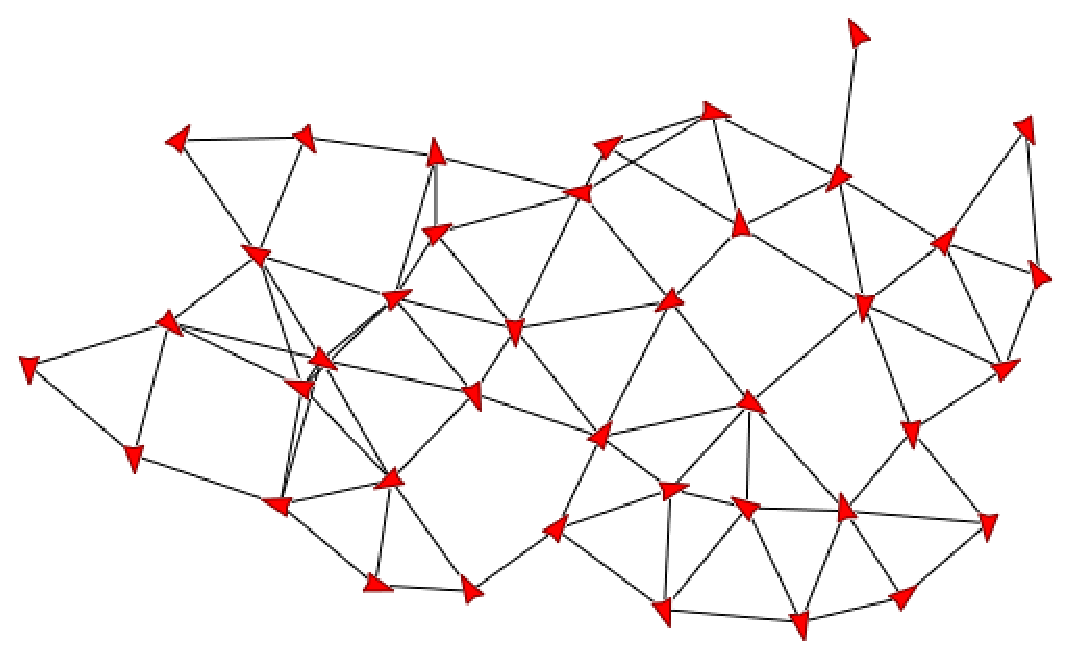
\includegraphics[width=0.9\textwidth]{figs/forty_sq_init}
        \end{minipage}
        \begin{minipage}{0.7\linewidth}
            \centering
            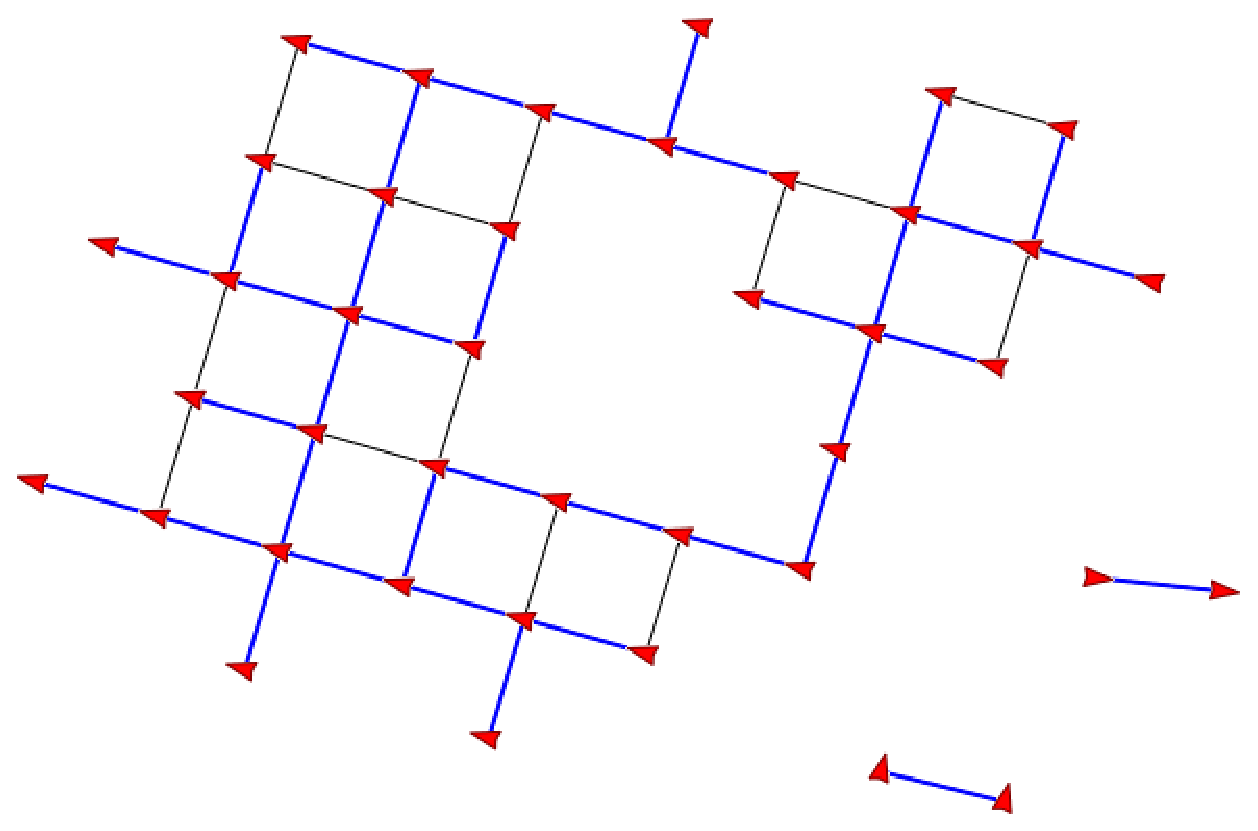
\includegraphics[width=0.9\textwidth]{figs/forty_sq_old}
        \end{minipage}
        \begin{minipage}{0.7\linewidth}
            \centering
            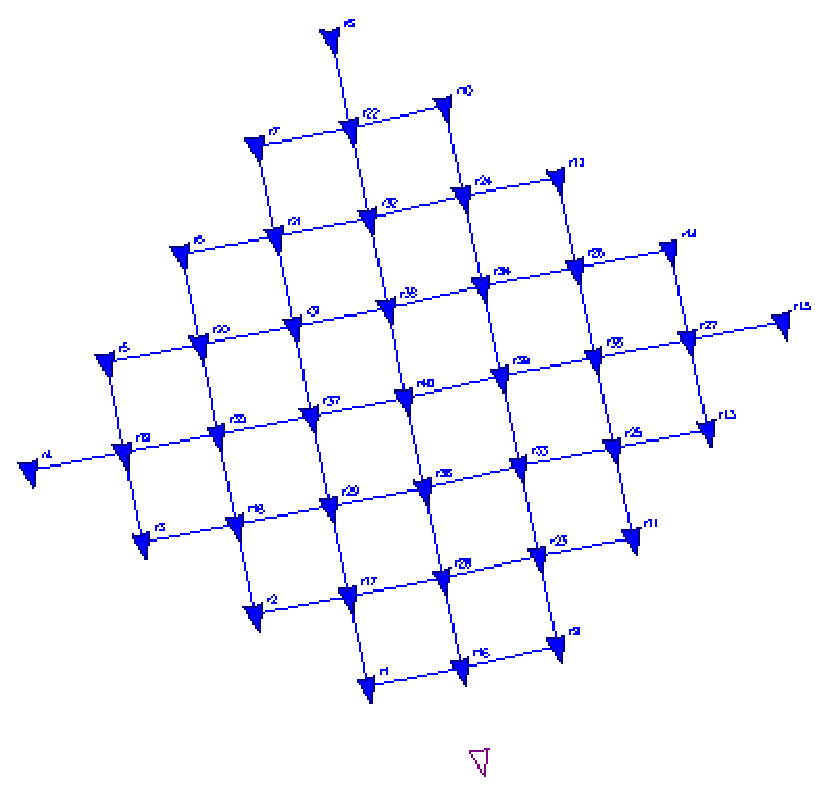
\includegraphics[width=0.9\textwidth]{figs/forty_sq_new}
        \end{minipage}
        \caption{[top] Initial poses of $40$ robots. [mid] Final formation using the primary algorithm in Chapter~\ref{chp:mrf1}. [bottom] Final formation using the new algorithm.}
        \label{fig:forty_sq_comp}
    \end{figure}

  On the other side, we are confident to get a better formation
  quality by executing the new algorithm, compared with the results of
  executing the old algorithm. 
  %
  A fact is that the new algorithm always outputs a
  deterministic combinatorial relationship of the given set of robots,
  regardless of the distribution of their initial poses. 
  %
  Therefore, these
  experimental statics show that the deviation of the fulfillment ratio
  is always zero when performing the new algorithm.


  Above all, there is a trade-off between the execution time and the
  formation quality when comparing the performance of two algorithms.
  %
  However, for the new algorithm, the execution time is proved bounded,
  but not for the old algorithm.


  
  %%%%%%%%%%%%%%%%%%%%%%%%%%%%%%%% 
  \begin{figure}
    \begin{minipage}[b]{0.9\linewidth}
      %trim=l b r t
      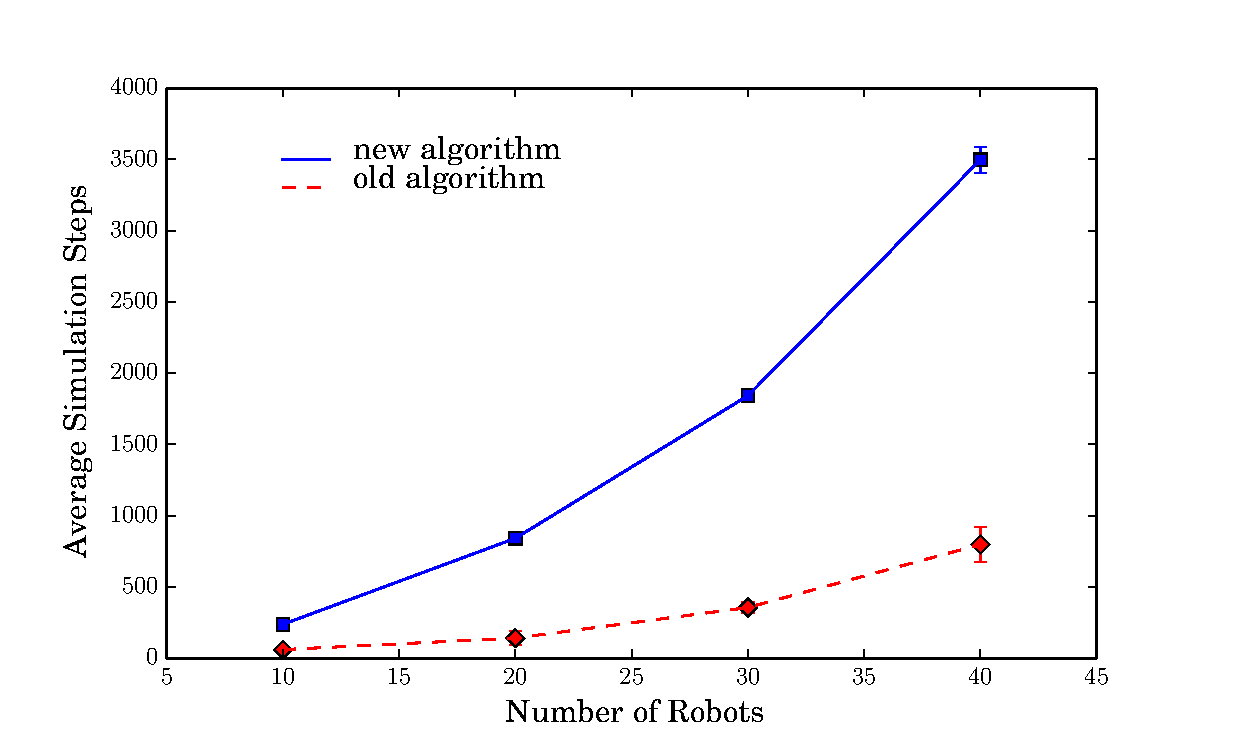
\includegraphics[trim=0.5cm 0cm 1.5cm 0,clip=true,width=\linewidth]{figs/steps_square}
    \end{minipage}
    \begin{minipage}[b]{0.9\linewidth}
      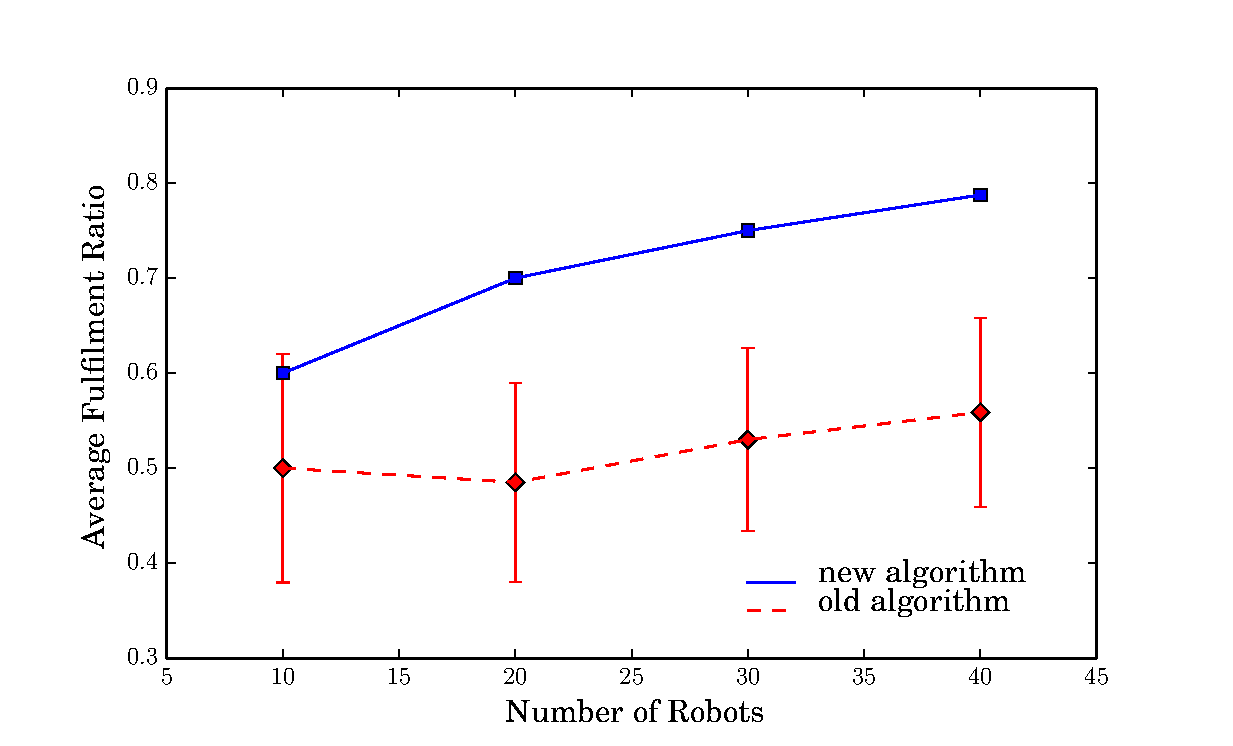
\includegraphics[trim=0.5cm 0 1.5cm 0,clip=true,width=\linewidth]{figs/ratio_square}
    \end{minipage}
    \caption{Repeated squares pattern: [top] The average execution time with deviation. [bottom] The average fulfillment ratio with deviation.}
    \label{fig:sq_comp}
  \end{figure}
  %%%%%%%%%%%%%%%%%%%%%%%%%%%%%%%%
 %%%%%%%%%%%%%%%%%%%%%%%%%%%%%%%%
  \begin{figure}
    \begin{minipage}[b]{0.9\linewidth}
      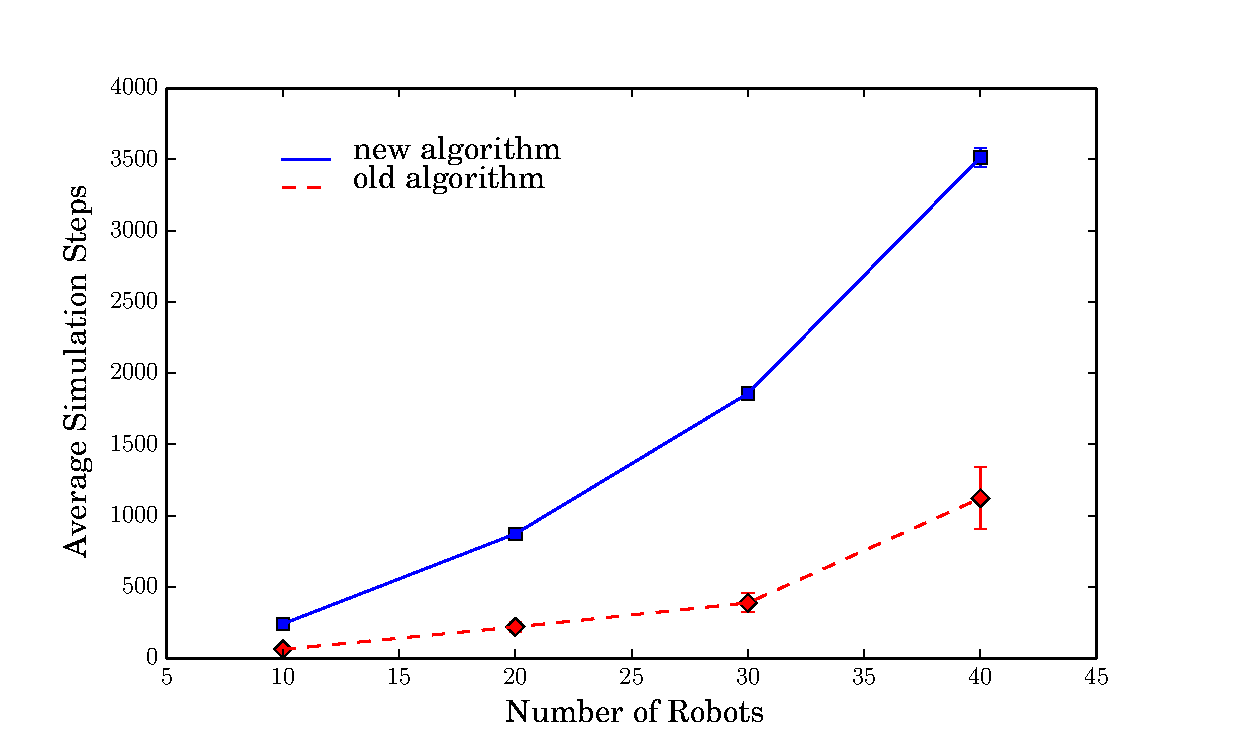
\includegraphics[trim=0.5cm 0cm 1.5cm 0,clip=true,width=\linewidth]{figs/steps_hexagon}
    \end{minipage}
    \begin{minipage}[b]{0.9\linewidth}
      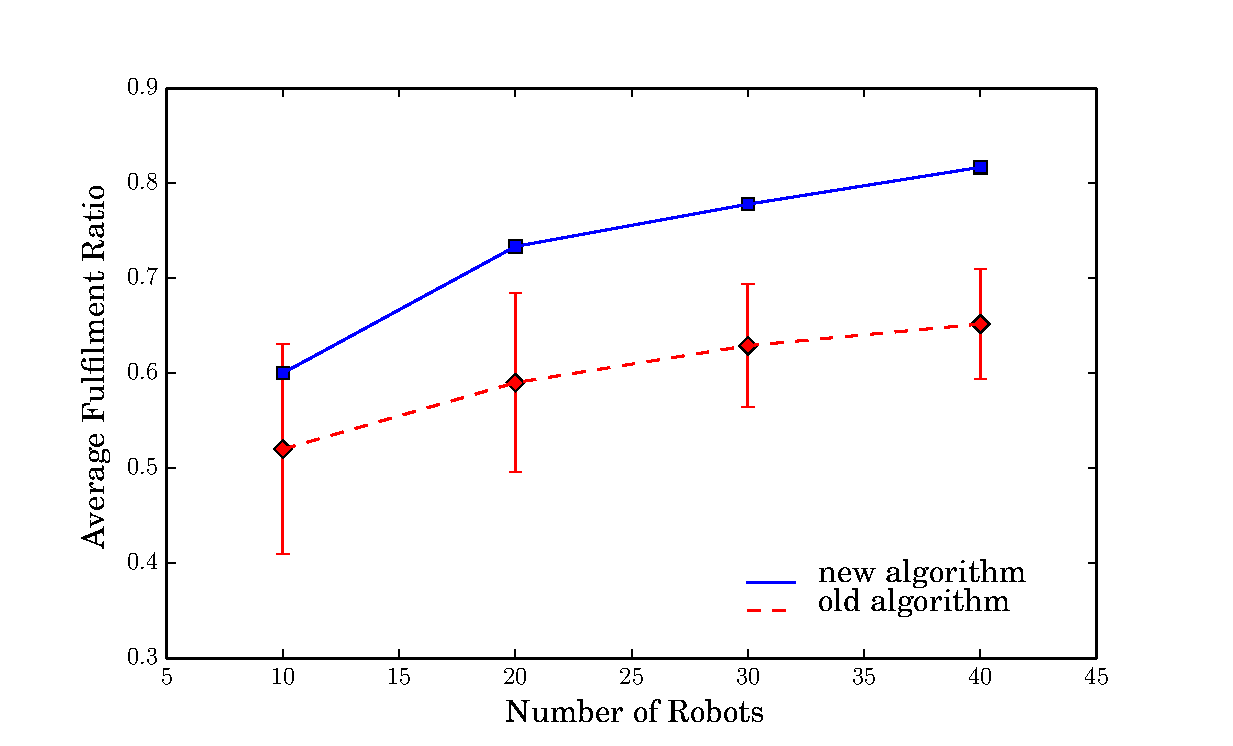
\includegraphics[trim=0.5cm 0 1.5cm 0,clip=true,width=\linewidth]{figs/ratio_hexagon}
    \end{minipage}
    \caption{Repeated hexagons pattern: [top] The average execution time with deviation. [bottom] The average fulfillment ratio with deviation.}
    \label{fig:hex_comp}
  \end{figure}
  %%%%%%%%%%%%%%%%%%%%%%%%%%%%%%%%
  %%%%%%%%%%%%%%%%%%%%%%%%%%%%%%%% 
  \begin{figure}
    \begin{minipage}[b]{0.9\linewidth}
      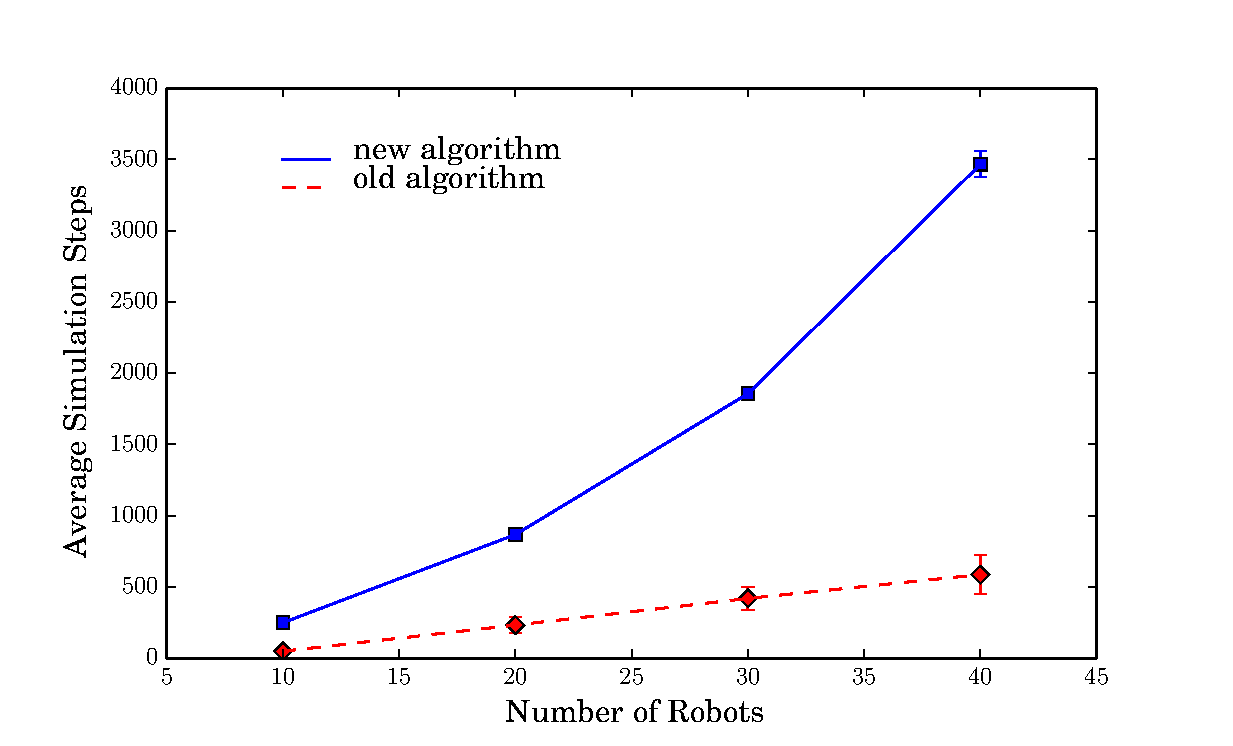
\includegraphics[trim=0.5cm 0cm 1.5cm 0,clip=true,width=\linewidth]{figs/steps_octagon_square}
    \end{minipage}
    \begin{minipage}[b]{0.9\linewidth}
      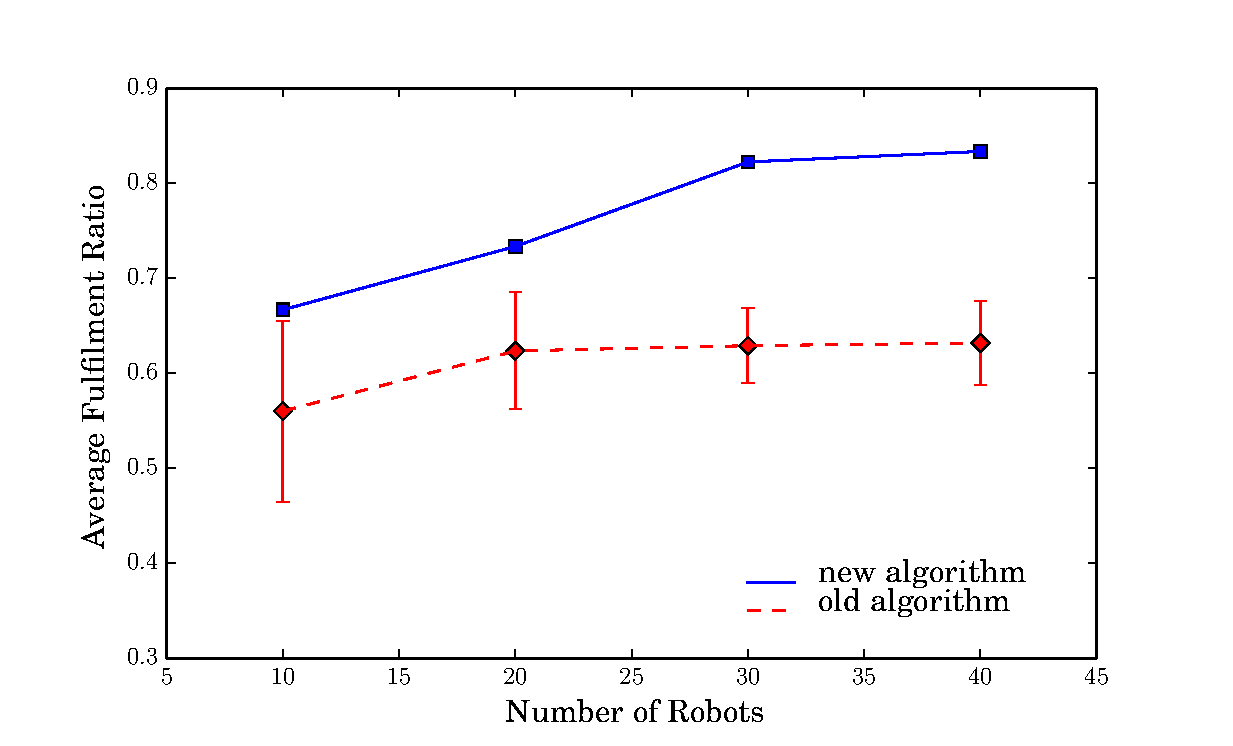
\includegraphics[trim=0.5cm 0 1.5cm 0,clip=true,width=\linewidth]{figs/ratio_octagon_square}
    \end{minipage}
    \caption{Repeated octagons and squares pattern: [top] The average execution time with deviation. [bottom] The average fulfillment ratio with deviation.}
    \label{fig:octsq_comp}
  \end{figure}
  %%%%%%%%%%%%%%%%%%%%%%%%%%%%%%%%
  
%\clearpage
\section{Conclusions}
\label{sec:conc-mrf2}

In this chapter, we have introduced the second type of decentralized formation algorithm for the problem in Chapter~\ref{chp:mrf}.
%
Compared with the method in Chapter~\ref{chp:mrf1}, we conclude that this algorithm is provably-correct in its bounded-time execution and improved formation quality notably.
%
Another feature of this algorithm is the NCLB motion strategy that maintains the connectivity of the communication graph during its execution.



However, there are two major limitations for this approach:
\begin{enumerate}
\item inefficient performance: each time only one robot moves to a vacancy, and the travel distance of each relocation process is far from optimal;
\item lack of the robustness and error-tolerance: in contrast to the primary algorithm, the new approach may encounter failures when some robots in the systems fail to work properly. Take Figure~\ref{fig:safedist2} as an example, if robot $r_4$ does not perform message passing or fails to move, then the desired lattice can not be formed correctly, and the algorithm will never terminate. 
Another scenario is that, when some new robots with IDs higher than any robot's ID in the system are added, the algorithm may not response well. Consider Figure~\ref{fig:forty_sq_comp}, the bottom figure has shown that forty robots already formed a repeating square pattern. If a new robot with its ID higher than any one is added to the network, then the robots can not re-organize themselves because there is no way for those stable robots to reset their status back to unstable.
\end{enumerate}




